\documentclass[a4paper,12pt]{article}
\usepackage[utf8]{inputenc}

\usepackage[brazil]{babel}
\usepackage[lmargin=3cm,tmargin=3cm,rmargin=2cm,bmargin=2cm]{geometry}
\usepackage{amsmath,amsthm,amsfonts,amssymb,dsfont,mathtools}
\usepackage{blindtext}
\usepackage[T1]{fontenc}
\usepackage{graphicx}
\usepackage{pgfplots}



\title{Projeto}

\author{LuizLamim}
\date{Outubro 2022}

\begin{document}

\maketitle

\section{Equações matemáticas \LaTeX}
\subsection{Introdução}
    Nesse artigo irei plotar alguns exemplos de gráficos com eixo x e y (duas dimensãoes), com eixo
x, y, e z (três dimensões), equações e algumas matrizes. O Objetivo principal é exemplificar algumas
funções do editor de texto \LaTeX. Tal ferramenta é fundamental no desenvolvimento de 
artigos científicos e trabalhos no campo da Engenharia de forma mais eficiente. Devido ao grande
número de possibilidades, formatações e pacotes da ferramenta é possível formar documentos complexos como será
mostrado a seguir. 

\begin{center}
\textbf{   Pacotes em \LaTeX (usepackages) são parecidos com bibliotecas em programação. 
    São conjuntos de funções específicas que devem ser previamente invocadas antes de serem utilizadas. 
    Um pacote ou biblioteca podem ser desenvolvido na liguagem de acordo com o surgimento de uma necessidade
    específica. Todo esse universo de possibilidades dá versatilidade ao autor. }
\end{center}

\subsection{Equações e plot de gráficos}

Esse é um exemplo de introdução de imagens no \LaTeX. É possível formatar o tamanho e indicar o local 
da imagem.

\begin{figure}[ht]
\centering
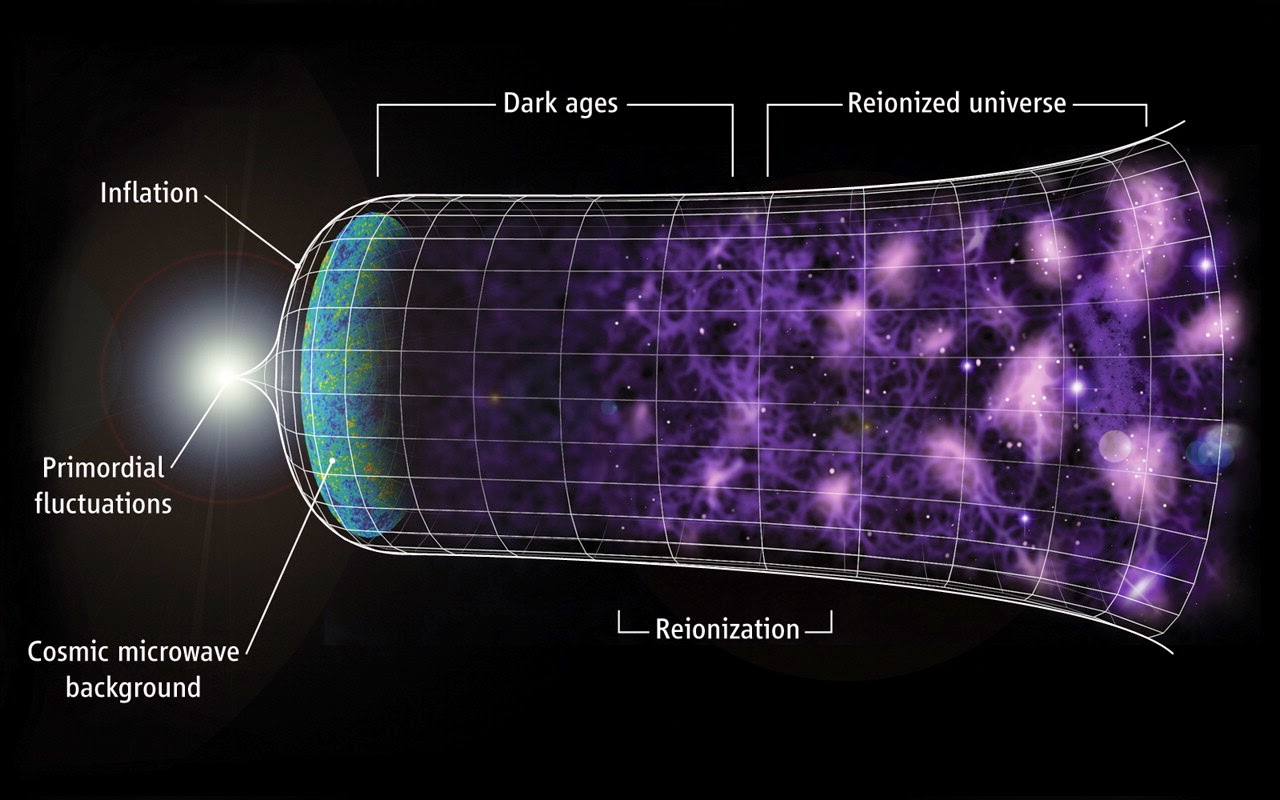
\includegraphics[width=10cm]{figuras/bigbang.jpeg}
\caption{Expansão do universo.}
\label{fig01}
\end{figure}




\newpage


\section{Criando uma Matrix no \LaTeX}
\begin{enumerate}
\item Considere a matriz
$
\begin{vmatrix}
    1 & 6 & 5 \\
    1 & 7 & 7 \\
    10 & 15 & 1

\end{vmatrix}
$ Calcule o que foi solicitado abaixo:
\begin{enumerate}
    \item $\det M$
    \item $M^{-1}$
    \item $M^T$
\end{enumerate}

\end{enumerate}

\section{Criando Equações no \LaTeX}
\subsection{Escrevendo Integrais com \LaTeX}

\begin{equation}
    \int_0^1 f(x)dx
\end{equation}

\subsection{Plotando gráficos 2D}


\end{document}